\vspace{-0.2in}

\section{Problem Statement}
\label{sec:Problem_Statement}

\vspace{-0.1in}
Consider a set of mixed-criticality component-based applications that are distributed and deployed across a cluster of embedded computing nodes. Each component has a set of interfaces that it exposes to other components and to the underlying framework. Once deployed, each component works by executing operations placed on its component message queue. Each component is associated with a single executor thread that handles these operation requests. These executor threads are scheduled in conjunction with a known set of highly critical system threads and low priority best-effort threads. Furthermore, the application threads are also subject to a temporally partitioned scheduling scheme. System assumptions include (1) knowledge of the sequence of computational steps of known duration that are executed inside each component operation, (2) knowledge of the worst-case estimated time taken by each computational step, and (3) the estimated worst-case time taken to initiate a remote function call and to process the response, accounting for network-level delays. Using this knowledge about the system, the problem here is to ensure that the temporal behavior of all the application components lies within the bounds laid out by the system specifications. Ideally, this is achieved by verifying such system properties as lack of deadline violations for component operations. For scenarios where the system design isn't complete, e.g. application thread priorities are unknown, the paper describes the utility of an approach to identifying the subset of system behaviors that satisfy timing requirements and provide useful information to designers, e.g. partial thread execution orders. 

\vspace{-0.2in}   

\section{Colored Petri net-based Modeling}
\label{sec:CPN_Modeling}

\vspace{-0.1in}

This section briefly describes how CPN can be used to build an extensible, scalable analysis model for component-based software applications. To edit, simulate and analyze this model, we use the CPN Tools \cite{CPNTools} tool suite. 

The CPN model captures the behavioral semantics of our component model described in \cite{ISIS_F6_ISORC:13}, using knowledge of several factors that resolve the deployment of the component-based application. These factors include the following system properties: (1) configuration of temporal partition scheduling on each node of the distributed system, (2) location of each component being deployed (which temporal partition and which computing node) (3) properties of the component executor threads (thread priority), (4) properties of timers (period and offset), and (5) component interactions and assembly (i.e. the 'wiring'). 

%\vspace{-0.2in}
\begin{figure}[t]
	\centering
	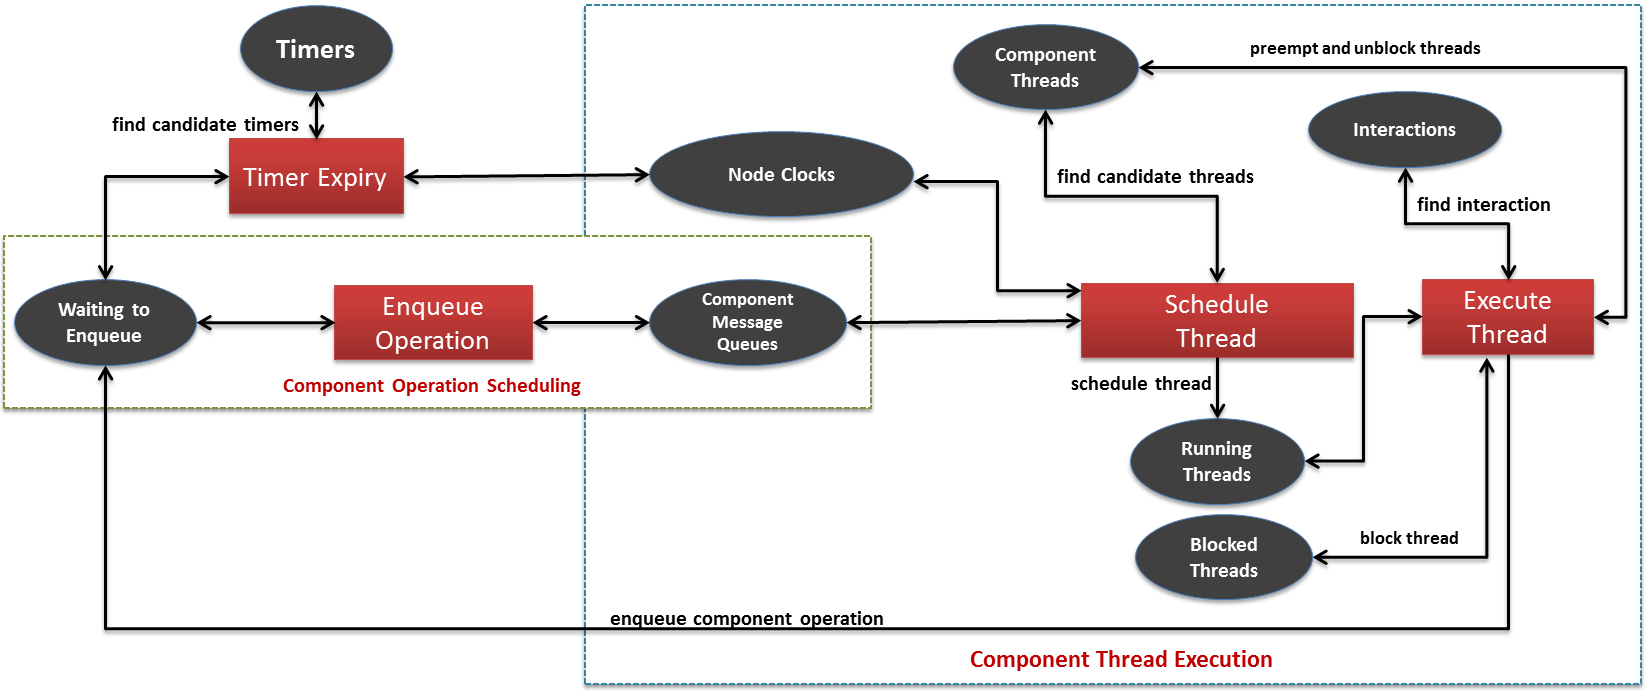
\includegraphics[width=\textwidth]{./figs/cpn_model}
	\caption{Hierarchical CPN Analysis Model}
	\label{fig:cpn_model}
	\vspace{-0.1in}
\end{figure}
%\vspace{-0.1in}

Figure \ref{fig:cpn_model} shows a top-level structure of the CPN-based analysis model. The place \emph{Component Threads} holds a token with a list of all executor threads responsible for component interactions. This list is maintained based on thread priorities on each node so that the highest priority ready thread is always chosen first by the OS scheduler. \emph{Timers} maintains a list of all infrastructural timers in the application. All timer expiries at a specific clock value\footnote{The clock values are integers.} are handled by the transition \emph{Timer Expiry}. A timer can be used in our component model to trigger the execution of a component operation. DREMS components are dormant by default.  Once initialized, a component executor is not eligible to run until there is an operation added to the component message queue. To start a sequence of component interactions, periodic or sporadic timers can be used to trigger an operation of a component.

If a timer triggers a component execution, this component is identified as a candidate for scheduling by \emph{Schedule Thread}. This transition always schedules the highest priority thread that is ready to execute in the active partition on each node. If two threads of equal priority are eligible, the scheduler picks one at random and maintains a round-robin scheduling scheme. If the highest priority thread is not already servicing an operation request, the highest priority operation from its message queue is dequeued and scheduled for execution.

The \emph{Component Message Queues} place is a list that manages the message queues of all components across all nodes. Every time a component thread executes an operation, the completion of this operation could trigger another component into execution. For instance - the completion of an RMI query on a client component triggers a server-side RMI operation that this server will have to execute. Such interactions are derived from the modeling tools and appropriate tokens are generated in place \emph{Interactions}. When executing component threads, \emph{Execute Thread} checks to see if the execution has any effect on the running thread or on other threads. Therefore, when the client thread completes an RMI query, this thread is moved to \emph{Blocked Threads} and a server RMI operation is placed in \emph{Waiting to Enqueue}. Later, when the server thread is scheduled, the client is unblocked appropriately.





